This chapter will give a review of the Deformable Parts Model as described in \cite{5255236}  and its implementation (VOC-release 3) on which this project builds upon. Section \ref{sec:ext3D} will then introduce the modifications that were made to extend it towards 3D. Wherever possible notation used in \cite{5255236} and \cite{6248075} will be adopted.

\section{DPM Review}\label{sec:dpmreview}
The DPM is a type of sliding window detector, consisting of a set of linear filters which are applied to a feature pyramid computed from an input image. Each DPM has a root filter which models the object appearance as a whole, and several higher resolution part filters which model smaller parts of the object. 

\subsection{Sliding Window Approach}
The idea behind the sliding window approach is that, given an input image and a window (of smaller size than the image), the window is placed on all locations inside the image and  for the region covered by the window to decide whether the object is present or not. 

Rather than working with images directly, feature maps are computed from them. A feature map G is a two-dimensional array of $d$-dimensional feature vectors. One can think of each feature vector as representing a small image patch and the feature map as a grid of feature vectors computed from image patches. The features used in \cite{5255236} are a modified version of the HOG features introduced in \cite{1467360}.
For now let us look at the case of a model consisting of a single root filter (e.g. a DPM without parts).  A root filter F is a two-dimensional array of $d$-dimensional weight vectors. The root filter can be interpreted as the "window" that slides through each position on the feature map to detect objects. 

To detect objects at different scales, a feature pyramid is used (see figure \ref{fig:pyra} and the appendix for a detailed description). The subsampling factor from level to level is constant and determined via a parameter $\lambda$ which fixes the number of levels in an octave. A feature map an octave beneath in the pyramid is computed at twice the resolution.

\begin{figure}[]
\begin{center}
        \begin{subfigure}[b]{0.49\textwidth}
                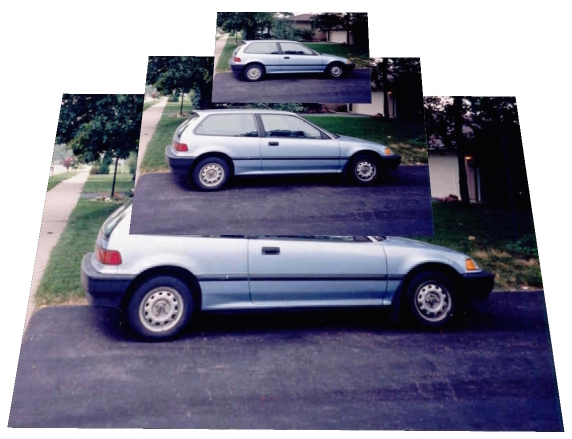
\includegraphics[width=\textwidth]{imagepyra}
                \caption{Image pyramid}\label{fig:impyra}
        \end{subfigure}
        \begin{subfigure}[b]{0.49\textwidth}
               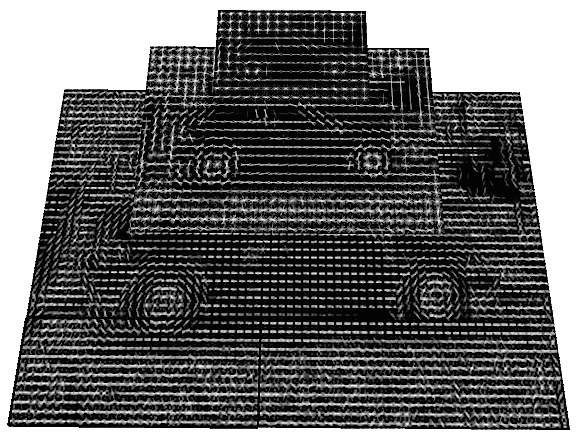
\includegraphics[width=\textwidth]{pyrahog}
               \caption{HOG feature pyramid}\label{fig:featpyra}
        \end{subfigure}
\caption{These figures illustrate image and feature pyramids. The pyramids here span two octaves with one level each. Therefore each pyramid level downwards doubles the image resolution. Note that the cell-size of all the feature maps in the HOG pyramid is constant.}
\label{fig:pyra}
\end{center}
\end{figure}


Each placement of the filter in the feature pyramid is assigned a score via the "dot"-product of the filter and the corresponding sub-array of the feature map at the given level. More formally: given a filter $F$ of size $w\times h$, a filter placement in the feature pyramid is defined by a three-tuple $p=(x,y,l)$ where $(x,y)$ specifies the position of the upper-left corner of the filter in the $l$-th level of a feature pyramid $H$. Further let $\phi (H,p,w,h)$ denote the vector obtained by concatenating the feature vectors in $H$, belonging to a window of size $w\times h$ at position $p$ in $H$.  The score of this placement is then given by:
\begin{equation}
score(p)=F' \cdot \phi (H,p)
\end{equation}
where $F'$ denotes the concatenation of the weight vectors in $F$ and $\phi (H,p)$ is a shorthand for $\phi (H,p,w,h)$, as $w$ and $h$ are implicit from $F$. 

\begin{figure}[]
\begin{center}
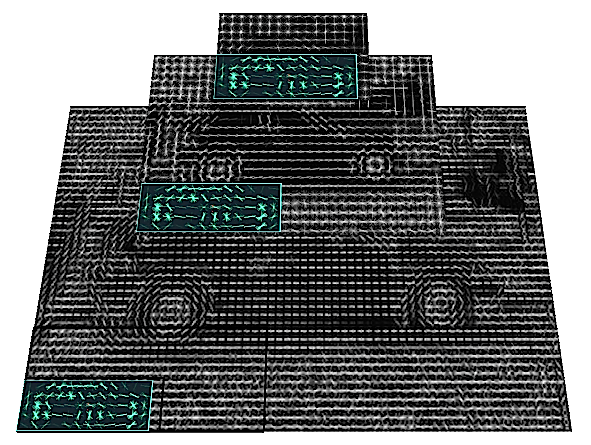
\includegraphics[width=0.6\textwidth]{rootInPyra}           
\caption{This figure illustrates the instantiations of a filter in a feature pyramid. The same filter is placed in the lower left corner of each pyramid level. To better distinct it from the feature maps, the filter is coloured. }
\label{fig:rootInPyra}
\end{center}
\end{figure}
 
\subsection{Deformable Parts and Mixture Models}\label{sec:defParts}
We will now extend the root-only model with parts and a deformation model. Let us consider the case of a DPM model for cars. The root filter approximately covers all of the car and models the object appearance as a whole. It also serves as a detection window. Part filters cover smaller, more detailed parts of the car, e.g. the tires or windows, and model their appearance at a higher resolution. The part filters are always placed $\lambda$ levels (an octave) below the root filter in the feature pyramid and are therefore computed at twice the resolution. Each part is placed at a fixed anchor-position relative to the root filter's position. This leads to a star-shaped model. To model intra-object class variations, parts  are allowed to deviate from their anchor positions by a certain amount restricted by a deformation cost.

Formally, a model with $n$ parts is defined by $(F_0,P_1,...,P_n,b)$ where $F_0$ is the root filter, $P_i$ is a model for part $i$, and $b$ is a bias term. $P_i$ in term consists of $(F_i, v_i, d_i)$ where $F_i$ is the part filter, $v_i$ specifies the anchor position, and $d_i$ is a four-tuple of coefficients for a quadratic  function modelling the deformation cost. A placement $z=(p_0,p_1,...,p_n)$ of all the filters in the feature pyramid is called a hypothesis. The displacement of the parts relative to their anchor position is given by $(dx_i,dy_i)=(x_i,y_i)-(2(x_0,y_0)+v_i)$. Remember that the parts are computed at twice the resolution of the root, hence the factor of two. Figure \ref{fig:anchor} illustrates part anchors and deformations.  Given the displacements, the deformation feature is set to $\phi_d (dx_i,dy_i)=(dx^2,dx,dy^2,dy)$. A hypothesis is assigned a score via
\begin{equation}\label{eq:score}
score(z)=\sum_{i=0}^n F'_i\cdot \phi(H,p_i)-\sum_{i=1}^n d_i\cdot \phi_d (dx_i,dy_i)+b.
\end{equation}
Note that the first term of the sum is concerned with the appearance and the second term with the deformation. 

\begin{figure}[]
\begin{center}
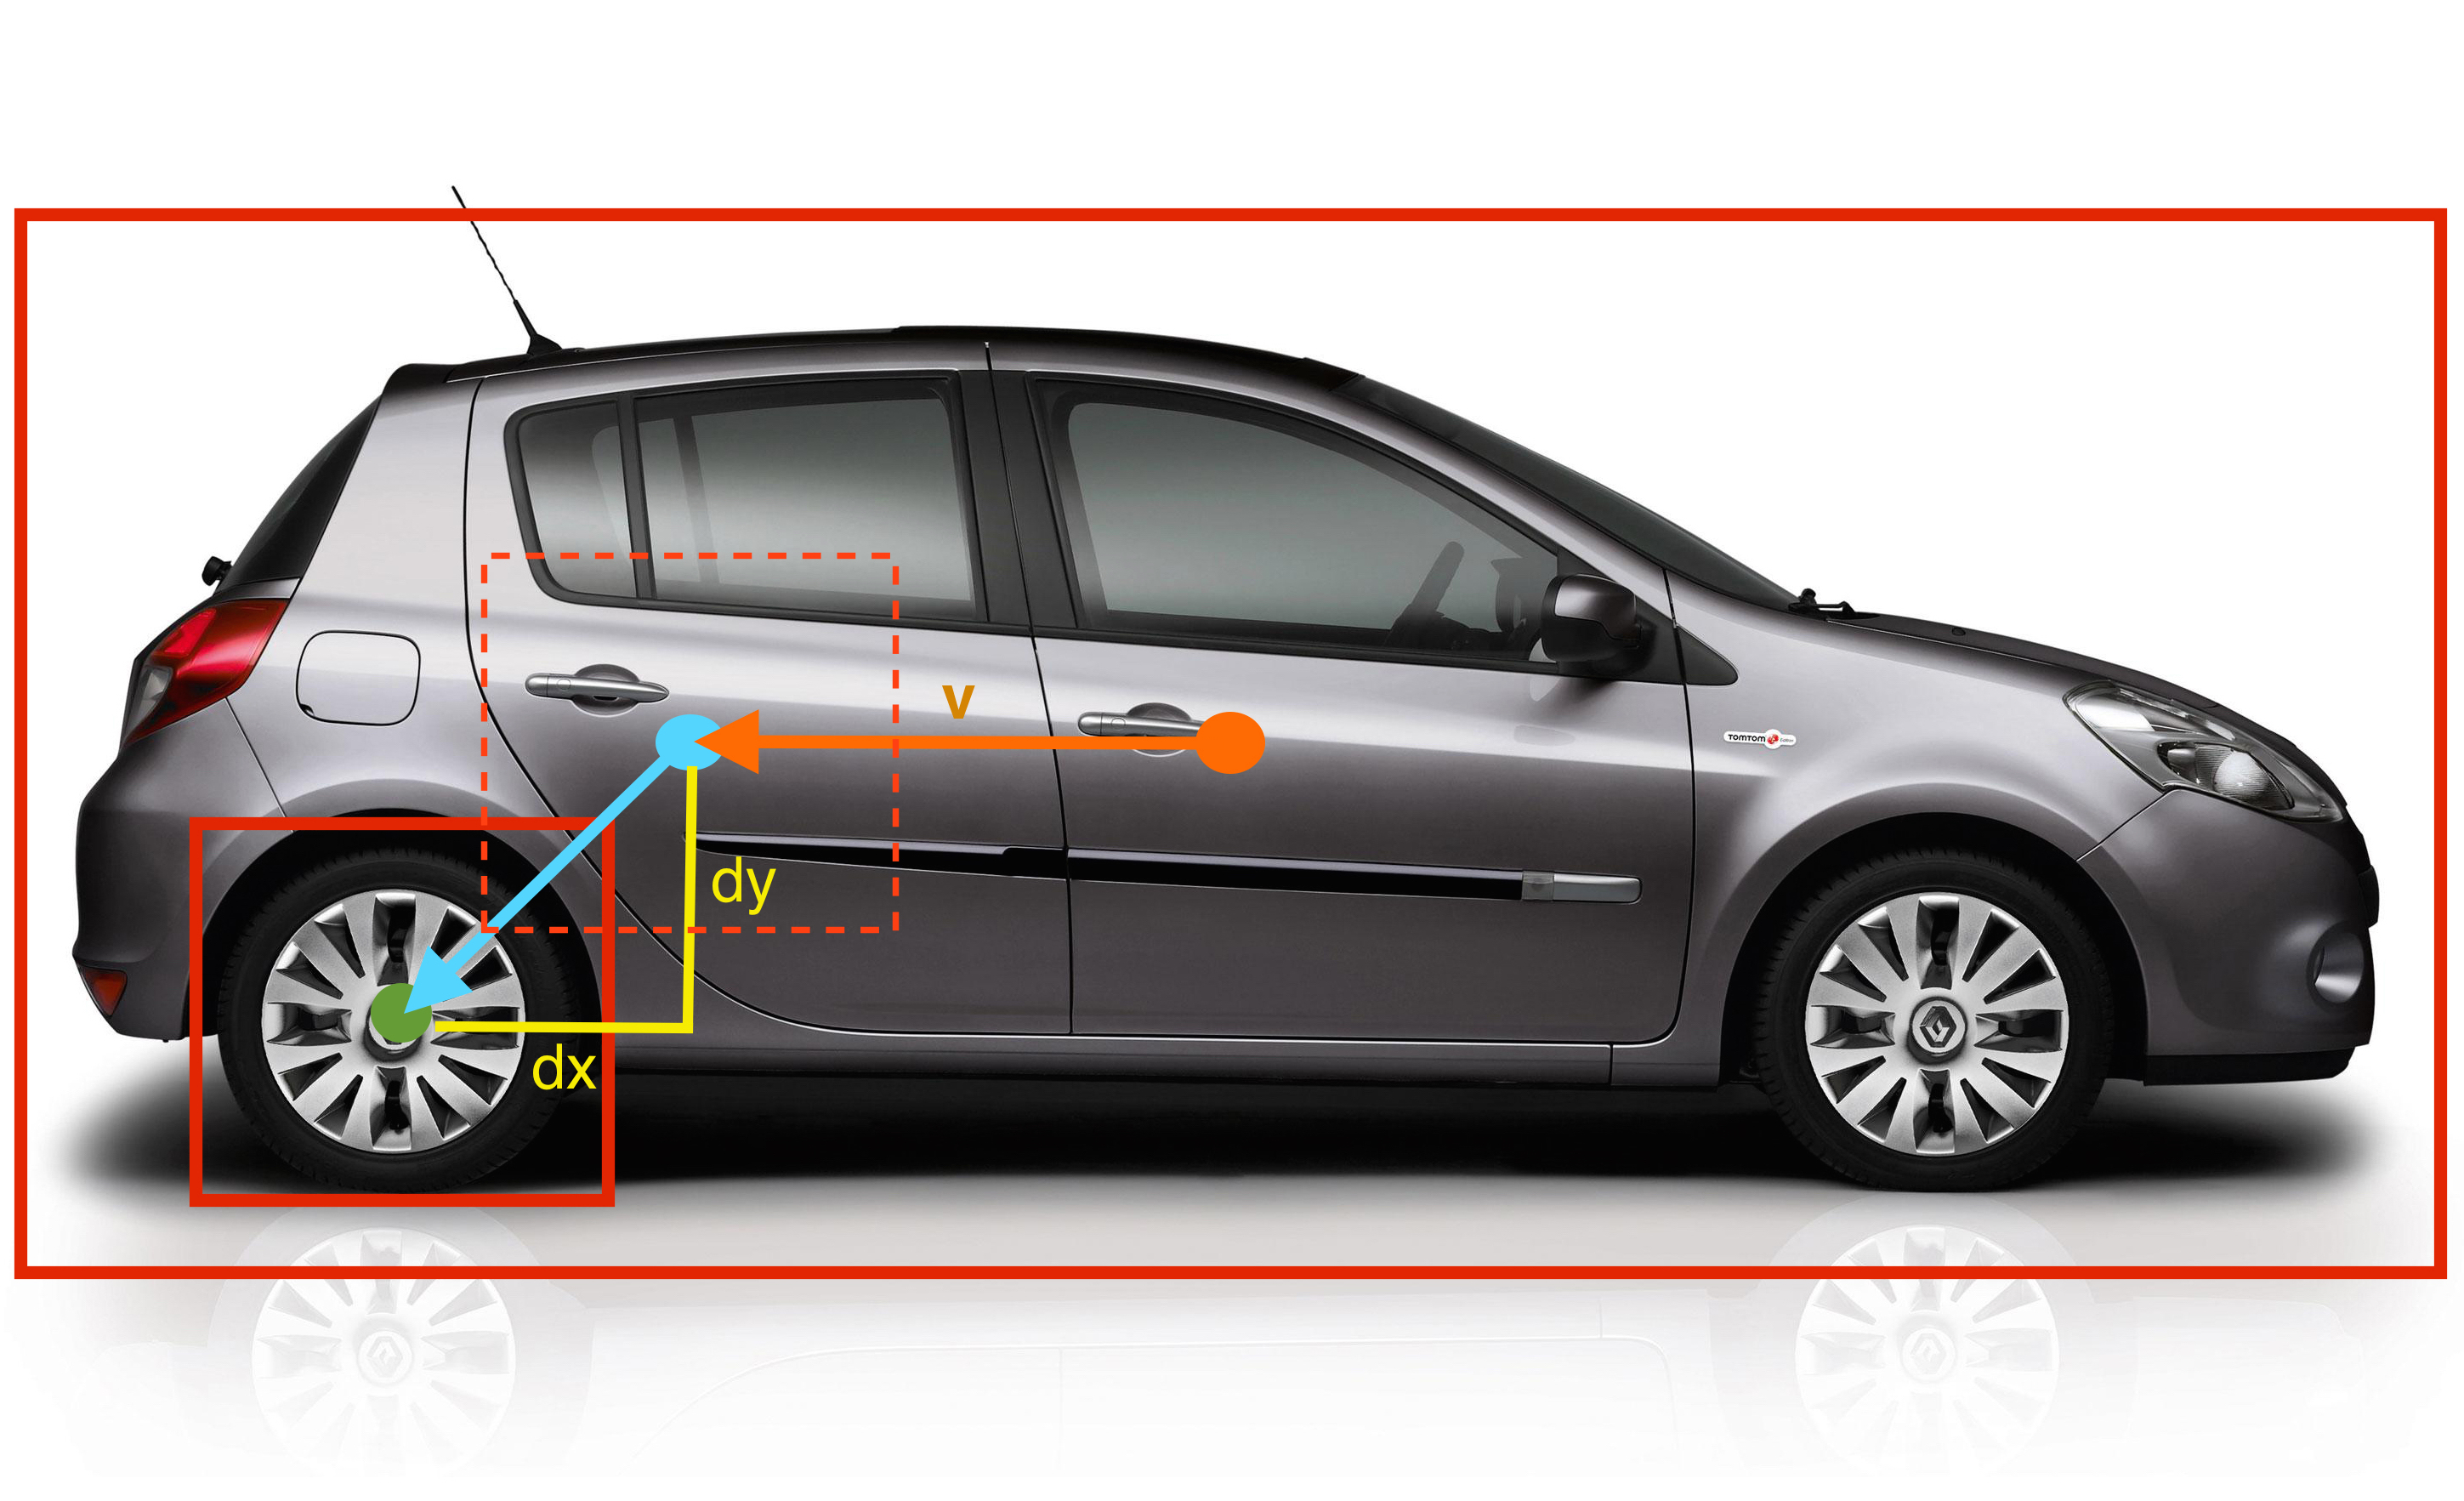
\includegraphics[width=0.8\textwidth]{anchor}           
\caption{This figure illustrates the anchors and displacements of the parts. The anchor position $v$ from the root centre  to the anchor is coloured in orange. The displacement from anchor to the part position is coloured in light blue.  }
\label{fig:anchor}
\end{center}
\end{figure}

To arrive at richer object models, several DPMs, as just described, are combined into one mixture model. A mixture model is an $m$-tupel $M=(M_1,...,M_m)$ where $M_c$ is the model for mixture-component $c$. An object hypothesis for a mixture model is given by $z=(c,p_0,...,p_{n_c})$ where $n_c$ specifies the number of parts in $M_c$ and the score for hypothesis $h$ is simply the score of $z'=(p_0,p_1,...,p_{n_c})$ for $M_c$.

By concatenating all the model-parameters of $M_c$ into a vector 
\begin{equation}
\beta_c=(F_0,F_1,...,Fn,d_1,...d_n,b)
\end{equation}
the whole mixture model can be  expressed through the vector $\beta=(\beta_1,...,\beta_m)$.
By similarly concatenating all the features of hypothesis $z'$ into a vector
\begin{equation}
\Phi(H,z')=(\phi(H,p_0),...,\phi(H,p_n),-\phi_d(x_1,y_1),...,-\phi_d(x_n,y_n),1)
\end{equation}
a sparse feature vector for hypothesis $h$ can be constructed by setting 
\begin{equation}
\Phi(H,z)=(0,...,0,\Phi(H,z'),0,...,0).
\end{equation}
The score of the hypothesis h can then be expressed via the dot product
\begin{equation}\label{eq:vecscore}
score(z)=\beta\cdot \Phi(H,z).
\end{equation}

\subsection{Inference}

As the root filters act as detection windows, the problem of object detection reduces to finding high scoring root placements. The score of a root placement for a mixture component is given by
\begin{equation}\label{eq:rscore}
score(p_0)=\max_{p_1,...p_n}score(p_0,p_1,...p_n).
\end{equation}
That is, for each root placement we want to find the best placements of all the parts. In practice, this is solved by first pre-computing the filter responses and storing them in an array $R_{i,l}(x,y)=F'_i\cdot\phi(H,(x,y,l)$ where $i$ specifies the filter and $l$ the level in the feature pyramid. The filter responses are then transformed via 
\begin{equation}\label{eq:dt}
D_{i,l}(x,y)=\max_{dx,dy}( R_{i,l}(x+dx,y+dy)-d_i\cdot\phi(dx,dy)).
\end{equation}
$D_{i,l}(x,y)$ gives the maximum contribution of part $i$ to a root filter placed in the feature pyramid so that the anchor position of part $i$ is at $(x,y,l)$. Given the array of filter responses, the maximum in equation \ref{eq:dt} can be computed in linear time using the efficient distance transform of sampled functions described in \cite{felzenszwalb2004distance}. The score \ref{eq:rscore} can now be expressed as
\begin{equation}
score(x_0,y_0,l_0)=R_{0,l_0}(x_0,y_0)+\sum_{i=1}^n D_{i,l_0-\lambda}(2(x_0,y_0)+v_i)+b.
\end{equation}

\subsubsection{Bounding Box Prediction}
To increase the accuracy of the detected bounding boxes, a technique called bounding box regression is used. The idea is to make use of the additional information provided by the part placements to refine the predicted bounding boxes. For one, parts allow to model intra-class variability better (e.g. a long car vs a short car) and parts are matched more precisely as they are modelled at twice the resolution of the root filter. 

After training a model, a separate bounding box predictor is trained. Let $g(z)$ be a feature vector obtained from the object hypothesis $z$ containing the width of the root filter in image coordinates and the upper left corners of each filter in image coordinates. The bounding box predictor is a linear function $b(g(z))=(x_1,y_1,x_2,y_2)$ of $g(z)$. The outputs of the function are the upper-left $(x_1,y_1)$ and lower-right corners $(x_2,y_2)$ of the predicted bounding box. The function $b$ is learnt using least-squares regression.

\subsubsection{Non-Maximum Suppression}
Using the bounding box prediction procedure as it stands now, typically leads to multiple overlapping detections as the model would detect the same object on locations that are spatially close to each other and have a similar scale. As simply choosing the highest scoring detection for each image would discard several correct detections on images that contain multiple object instances, another method to reduce detections is needed. 

With non-maximum suppression, detections are first sorted according to their score and the highest scoring detection is chosen. Greedily, more detections are chosen while skipping detections that overlap by more than 0.5 with a previously chosen detection.

\subsection{Training}

For training, a set of training examples $D=\{(x_1,y_1),...,(x_n,y_n)\}$ is given. The $x_i$'s are images and $y_i=(y_l,y_b)$ are labels where the label $y_l\in\{-1,1\}$ specifies whether the object is present or not and $y_b=(x_{min},y_{min},x_{max},y_{max})$ specifies a bounding box around the object in image coordinates. 

Let $Z(x,y)$ denote the set of possible latent hypothesis values for an example $x$ and labels $y$. For positive examples, $Z(x,y)$ is restricted to hypotheses which yield a root placement that overlaps with the bounding box label by at least $0.7$. For negative examples or during testing, no restrictions are set on $Z(x)$. Given a model $\beta$, equation \ref{eq:vecscore} allows to train a linear classifier 
\begin{equation}
f_\beta(x)=\max_{z\in Z(x,y)}\beta\cdot\Phi(x,z)
\end{equation}
using a formalism called Latent-SVM introduced in \cite{5255236} which is mathematically similar to MI-SVM \cite{andrewssupport}. Latent-SVM minimizes the objective function
\begin{equation}\label{eq:svm}
L_D(\beta)=\frac{1}{2}\|\beta\|^2+C\sum_{i=1}^n\max(0,1-y_if_\beta(x_i))
\end{equation}
in analogy to standard linear SVMs with standard hinge loss. This optimisation problem is semi-convex that is, given fixed latent variables for positive examples, it becomes convex. 

In practice equation \ref{eq:svm} is solved by repeatedly:
\begin{enumerate}\label{proc:train}
  \item Constructing a training set $D(Z')$ where $Z'$ fixes latent variables for both positive and negative examples while keeping $\beta$ fixed. Latent variables of positive examples are fixed by  finding $\argmax_{z\in Z(x,y)}\beta\cdot\Phi(x,z)$. For negative examples, hard negative mining is used. Concretely, we search for examples with $\beta\cdot\Phi(x,z)>-1.05$.
  \item Updating $\beta$ by solving \ref{eq:svm} on the constrained set via a gradient descent algorithm using sub-gradients similar to \cite{shalev2011pegasos}. 
\end{enumerate}

\begin{figure}[]
\begin{center}
        \begin{subfigure}[b]{0.45\textwidth}
                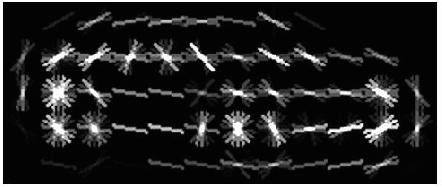
\includegraphics[width=\textwidth]{carhog_random}
                \caption{Initialised root filter after training against random negatives}
                \label{fig:carhog_random}
        \end{subfigure}
        \begin{subfigure}[b]{0.45\textwidth}
               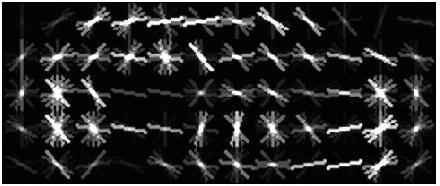
\includegraphics[width=\textwidth]{carhog_hard}
               \caption{Root filter after training against hard negatives}
                \label{fig:carhog_hard}
        \end{subfigure}
        \begin{subfigure}[b]{0.45\textwidth}
               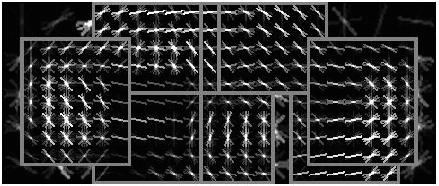
\includegraphics[width=\textwidth]{carhog_partinit}
               \caption{Mixture component after parts have been initialised}
                \label{fig:carhog_partinit}
        \end{subfigure}
        \begin{subfigure}[b]{0.45\textwidth}
               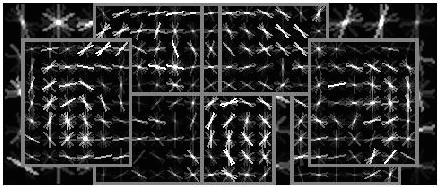
\includegraphics[width=\textwidth]{carhog_final}
               \caption{Mixture component after training against hard negatives}
                \label{fig:carhog_final}
        \end{subfigure}
\caption{This figure visualises the evolution of a mixture component of an eight viewpoint 3D DPM during the training procedure.}
\label{fig:carhog}
\end{center}
\end{figure}

\subsection{Initialisation}
An $n$-component model is initialised by first splitting the positive training examples according to aspect ratio statistics in $n$ training-sets,  and then training root filters for each component. Root filter dimensions are chosen in a way that their covered area is not greater than 80\% of the positive bounding boxes. Root filters are trained by warping positive bounding boxes to filter dimensions and training against negative examples obtained by extracting features from randomly selected regions of negative training images. Once all the root filters are initialised, the model is trained using several iterations of hard negative mining. Note that at this stage, only the component variable and root placement is treated as latent. 

The part filters are initialised by placing them on high "energy" regions, that is, regions with high euclidean norm of positive root filter weights. Possible part shapes are chosen from a pool of shape-templates and greedily added to the model. Regions covered by a part are zeroed out in the energy map and the next part is chosen until a fixed number of $k$ parts are added. In \cite{5255236} symmetry constraints on both the root and parts, are placed. Root filters are constrained to be symmetric along the vertical axis, as are parts lying on the centre vertical axis. Parts not lying in the centre have a symmetric partner.


\section{Extension to 3D}\label{sec:ext3D}
To extend the DPM to 3D, this project largely followed the approach of \cite{6248075} and \cite{Pepik:2012aa}. Training a 3D DPM relies highly on having viewpoint annotated training data. The model presented here is trained by using both real and synthetic training examples of cars. The synthetic examples were obtained by renderings of CAD models onto negative training images or backgrounds of mean pixel colour of the training images (see figure \ref{fig:CAD}). Experiments with both, orthographic and perspective projections for the rendering were done. Both \cite{6248075} and \cite{Pepik:2012aa} rely on rendered CAD models as well, but  they use non-photorealistic gradiant-based renderings and projective projections. For real training data, positive examples from the 3D object dataset \cite{4408987} and examples from VOC2012 \cite{pascal-voc-2012} with viewpoint annotations provided by \cite{xiang_wacv14} were used. 

\begin{figure}
\begin{center}
        \begin{subfigure}[b]{0.49\textwidth}
                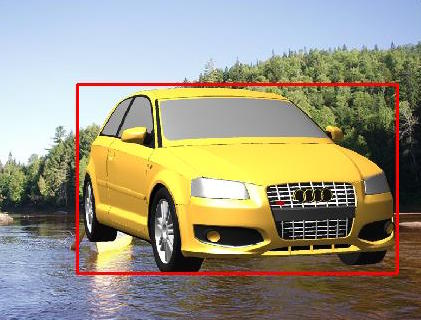
\includegraphics[width=\textwidth]{CADexample}
        \end{subfigure}
        \begin{subfigure}[b]{0.49\textwidth}
               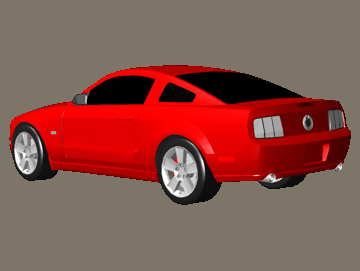
\includegraphics[width=\textwidth]{CADblack}
        \end{subfigure}
\caption{A CAD example rendered on a negative training image including the annotated bounding box (left). And a CAD example rendered on a background of mean pixels (right). Both were rendered using perspective projection.}
\label{fig:CAD}
\end{center}
\end{figure}

All the symmetry constraints placed on the root and parts from the original DPM \cite{5255236} were eliminated as they do not allow to distinguish different views (mirrored left and right side views of a car look identical). Figure \ref{fig:carhog} shows the evolution of one model view during the training procedure.


\subsection{Assigning Components to Viewpoints}
The first modification to the model was to relate mixture components to specific viewpoints. To achieve this, the training data $D$ was split according to viewpoint annotations into $n_c$ component training sets $\{D_i\}_{i=1}^{n_c}$ and root filters were initialised on each of these sets by training against random negatives (see figure \ref{fig:carhog_random}). Three parameters control the splitting of the training set: 
\begin{itemize}
  \item $n_c$: specifies the number of mixture components.
  \item $n_a$: specifies the number of different azimuth angles.
  \item $n_e$: specifies the number of different elevations. 
\end{itemize}
Note that $n_c=n_a\cdot n_e$. Viewpoints are split evenly across components, i.e. a model with $(n_c, n_a, n_e)=(16,8,2)$ would have eight azimuth angles lying in $\{0,45,90,135,180,225,270\}$. In this project a setting of $n_e=1$ was most often used while only varying $n_c$. Setting $n_e=2$ doubles the complexity of the model while only giving slight, if any, improvement in performance. Also, viewpoint accuracy as measured in  \cite{xiang_wacv14} only considers correct azimuth angle binning and example images from from VOC2012 \cite{pascal-voc-2012} typically don't vary much in elevation (see figure \ref{fig:hist}).

\begin{figure}
\begin{center}
        \begin{subfigure}[b]{0.49\textwidth}
                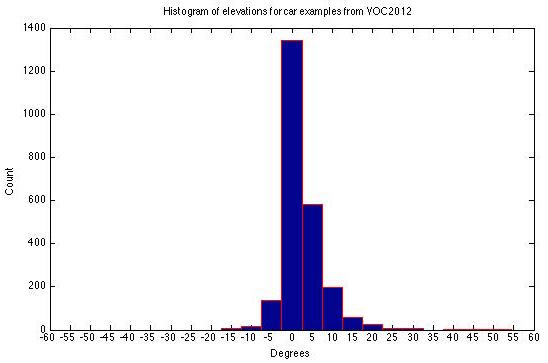
\includegraphics[width=\textwidth]{carElevHist}
        \end{subfigure}
        \begin{subfigure}[b]{0.49\textwidth}
                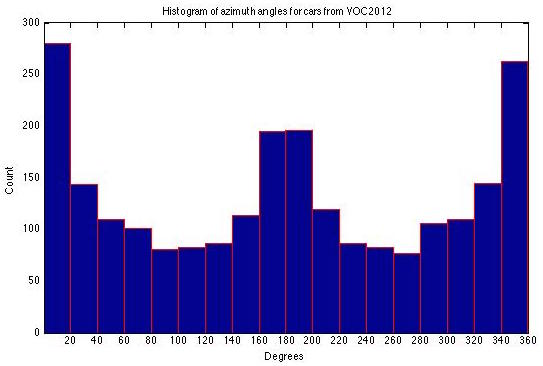
\includegraphics[width=\textwidth]{azimuthHist}
        \end{subfigure}
\caption{Histograms showing the distribution of elevations (left) and azimuth angles (right) across car examples from VOC2012 as annotated by \cite{xiang_wacv14}.}\label{fig:hist}
\end{center}
\end{figure}

During latent training, if a positive example falls within an angle $\Delta\alpha$ of a viewpoint assigned to a mixture component $c$, the latent component label is restricted to $c$. This has the nice side-effect of speeding up training as we do not have to search over all the components. Choosing $\Delta\alpha$ leads to a trade-off between precision and viewpoint accuracy. A value of $\Delta\alpha\in[10,...,20]$ was found to perform well. 

Another way of enforcing the correct component label during training is to introduce a penalty for incorrect viewpoint predictions. Formally, the labels of positive examples are extended by a component label $y_c$ leading to $y=(y_l,y_b,y_c)$. During latent positive search, latent variables would then be set to:
\begin{equation}\label{eq:penalty}
 z'=\argmax_{z\in Z(x,y)}(\beta\cdot\Phi(x,z)-l(y_c,c))
\end{equation}
where $l(y_c,c)=\mathbbm{1}{ [y_c\neq c] *\gamma}$ is the penalty term and the parameter $\gamma$ controls the weight of correct viewpoint assignments. The value of $\gamma$ was set to $\gamma=\max(1,\beta\cdot\Phi(x,z)/2)$. This way, very confident hypotheses are penalised more if they lead to wrong viewpoint estimates.  Experiments showed that this generally doesn't decrease detection performance while increasing viewpoint accuracy. 

\subsection{Placing Parts in 3D}
Going from 2D to 3D, anchor positions should now be placed in 3D object space rather than in the 2D root filter. As a reference coordinate system, a 3D object box is created and the origin is placed at the centre of the 3D box (see section \ref{sec:partInit} for details). Analogous to \cite{6248075}, parts are parametrised by part boxes $b_i=(s_{x_i},s_{y_i},s_{z_i})$ co-aligned with the object box. The new anchor position $v_i=(x_i,y_i,z_i)$, now in 3D, specifies the center of the part box in object coordinates. 

Part filters remain 2D templates of weight vectors and are sized so that they tightly cover the 3D part box as seen from the viewpoint of each mixture component. Mapping the 3D anchor positions to root filter coordinates is done by using an orthographic projection $P_c$ given by the viewpoint of component $c$. 

To make sure that part filters are learned consistently across views, latent part positions have to be inferred in 3D and simultaneous for all views of a given car model. This is achieved by making use of the CAD training data. Concretely, positive CAD examples are labeled with a model-ID $y_o$ and  a set $D(i)=\{(x,y)\in D:y_o=i\}$ is created. As CAD examples come with perfect annotations, the root placement and component variable are fixed. The root placement $p_c$ of component $c$ is chosen such that it yields maximum overlap with the annotated bounding box $y_b$. An object hypothesis in 3D is now defined by $h=(q_1,\ldots,q_n)$ where $q_i=(x_i,y_i,z_i)$ specifies the position of part $i$ in object coordinates. Note that for model component $c$ we get $z=(c,p_c,P_c(q_1),\ldots,P_c(q_n))$, the connection to the 2D hypothesis. Parts are still fixed to be an octave below the root filter in the feature pyramid. Let $\Psi(x,y,h)=\Phi(x,z(y,h))$, where $z(y,h)=(y_c,p_c,P_c(q_1),\ldots,P_c(q_n))$. The objective is now to find:
\begin{equation}\label{eq:3dConstraints}
	h'=\argmax_{h}(\sum_{(x,y)\in D(i)}\beta\cdot\Psi(x,y,h))
\end{equation}
Note that part displacements are still modelled in 2D (as in the model of \cite{6248075}) and are only dependent on other views via equation \ref{eq:3dConstraints}. This is in contrast to \cite{Pepik:2012aa} where displacements are modelled in 3D. While the 3D deformation model increases the models performance on ultra-wide baseline matching experiments, performance decreased for both detection and viewpoint estimation.

For each car model $i$ the procedure to solve \ref{eq:3dConstraints} is the following:
\begin{description}
  \item[1. Step]  Construct a 3D grid of possible part placements by padding the 3D object box to all sides. Padding is used to allow parts to move out of the 3D object box. 
  \item[2. Step] Compute feature maps for root and part filters for all examples $(x,y)\in D(i)$. The feature maps are computed so that they cover the whole 3D grid as seen from viewpoint $y_c$ and the fixed root placement yields maximum bounding box overlap.
  \item[3. Step] Iterate each part $p_j$ through each position $q_i$ of the 3D grid and sum up the scores for placing part $p_j$ at position $q_i$ for all the views. For a view related to component $c$, the score is given by  the score of placing it at $P_c(q_i)=(x_i,y_i)$ in root filter coordinates. That is, $score(p_j,q_i,c)=F'_j\cdot \phi(H,P_c(q_i))-d_j\cdot \phi_d (dx_j,dy_j)$. Note that here $H$ denotes the feature maps computed in step 2 and not a feature pyramid as in section \ref{sec:defParts}. The total score for placing $p_j$ at $q_i$ is then given by $score(p_j,q_i)=\sum_cscore(p_j,q_i,c)$.
  \item[4. Step] Pick the position that yields the highest overall score for each part. We set $h'=(\argmax_{q}score(p_1,q),\ldots,\argmax_{q}score(p_n,q))$.
\end{description}

Positive training examples for which no model-ID is provided, are treated as before, i.e. projecting the 3D anchor position to 2D and then searching for the best hypothesis in 2D. 

\subsection{Initialising Parts in 3D}\label{sec:partInit}

The initialisation of parts in 3D follows a similar heuristic as the 2D DPM by greedily placing them on high energy regions in 3D. For initialising a model with $m$ parts, the procedure is the following:  \begin{description}
  \item[1. Step] First the 3D object box is created which will be used to set up a grid of possible part placements. The box is modelled as 3D array of zeros. The dimensions of the box are initialised from the dimension of front and right view root filters. The height is set to twice the height of the front filter. The front and right view dimensions are then warped to fit the height of the box while preserving the aspect ratios. 
  \item[2. Step] Next, a pool of possible 3D part boxes $b_i=(s_{x_i},s_{y_i},s_{z_i})$ is created. Each part box is sized so that its volume approximately covers $1/m$ of the object box volume, concretely: $V_{part}=0.8*\frac{V_{object}}{m}$. 
  \item[3. Step] Each part box is then convolved with the 3D object box to get a grid of possible part placements. The part box is then moved through the grid and each grid position is assigned an energy. The energy of a grid position $q=(x,y,c)$ is obtained by projecting $q$ onto the root filters of all the components and then summing up the norm of positive root filter weights covered by the part box for all the components.
  \item[4. Step] The highest scoring shape and position combination is then chosen as new 3D part. To get non overlapping parts, regions covered by the new part are set to $-100$ in the 3D object box. This way, convolving the object box with the part shapes in step 3 gives grid positions that lead to overlapping parts a negative energy.
  \item[Repeat Step 3 and 4 until $m$ parts are chosen] 
\end{description}

As not all of the 3D parts are visible from all the views, only a maximum of $k$ parts are assigned to each view. For each view, parts are chosen greedily based on both their energy on the root filter and their depth in the 3D object box as seen from this view (parts in front are preferred). When a 3D part gets chosen, the region it covers is zeroed out in the root filter energy and a next part is chosen until either all $k$ parts are chosen or no more regions of the root energy can be covered by other parts (Note that different components might now have a different number of parts assigned to them). Part filters are chosen such that they tightly cover the 3D part box as seen from that view (see figure \ref{fig:3dbox}).

\begin{figure}
\begin{center}
           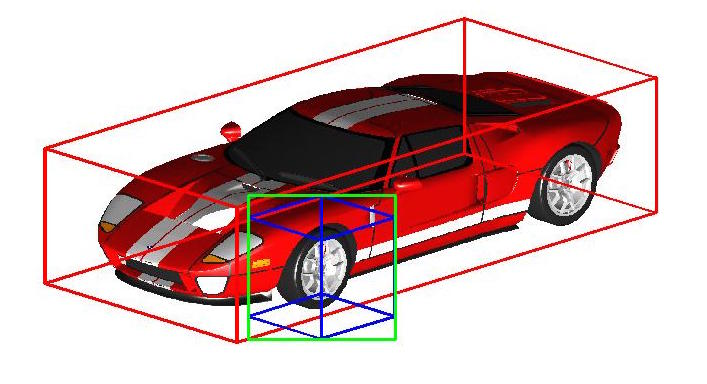
\includegraphics[width=0.8\textwidth]{3dbox}
\caption{This figure illustrates the idea of the 3D object box and the part parametrisation. The blue box represents a 3D part box and the green 2D box represents the part filter template from the given viewpoint.}
\label{fig:3dbox}
\end{center}
\end{figure}


\section{CNN Features}\label{sec:cnnFeat}
This section covers the steps taken to replace the HOG features of the original DPM with CNN features. The features used in this project are computed using the MatConvNet toolbox \cite{arXiv:1412.4564}. The concrete net used was the fast CNN-F architecture described in \cite{Chatfield14}. The net consists of 5 convolutional layers, some of which are followed by max-pooling layers, and 3 fully connected layers. The architecture used is similar to the one by Krizhevsky et al. \cite{krizhevsky2012imagenet} with the difference of having dense connectivity between convolutional layers in CNN-F and less convolution kernels in layers 1 (64 vs.96) and layers 3 and 4 (256 vs 384 each).

The standard input of CNN-F is a fixed sized $224\times224\times3$ image patch which is preprocessed by subtracting the mean training image. Constructing the feature pyramid requires to compute features for several rescaled versions of images of variable size. This project therefore used arbitrarily sized images as input to the CNN and approximated the normalisation by subtracting the mean pixel value from the input image. This approach was also used and experimentally justified in \cite{DBLP:journals/corr/IandolaMKGDK14} on the Caffe net \cite{jia2014caffe}. CAD examples were rendered on a background of the same mean pixels (see figure \ref{fig:CAD} right). 

Only the first five convolutional layers of the network are used to compute features (also discarding the last max-pooling layer). The output of the fifth convolutional layer given an input image of size $224\times224\times3$ is a feature map of size $13\times13\times256$. To get a more convenient mapping from image coordinates to feature map, the inputs of all the convolutional and max-pooling layers with kernel size $k$ are padded by $\lfloor k/2\rfloor$ with zeros to all sides (see table \ref{tab:cnn}). The output of a $224\times224\times3$ is then a $14\times14\times256$ feature map and coordinates $(x,y)$ in the feature map, map to $(16x,16y)$ in image coordinates (16 is the stride of the features computed by the fifth convolutional layer). For HOG features, the mapping was given by $(8x,8y)$ where 8 is the HOG cell size. This approach is similar to the one of \cite{girshick2014deformable} and was found to work slightly better than simply padding the feature maps to obtain the same mapping (used in \cite{DBLP:journals/corr/IandolaMKGDK14} and \cite{savalle8deformable}).

\begin{table}
\begin{center}
\begin{tabular}{|c||c|c|c|c|c|c|c|}
\hline
Layer & conv$_1$ & pool$_1$ &  conv$_2$ & pool$_2$ & conv$_3$ & conv$_4$ & conv$_5$ \\
\hline \hline
\#Filters & 64 & - & 256 & -& 256 &  256 &  256 \\
\hline
Size	& $11\times11$ & $3\times3$ & $5\times5$ & $3\times3$ &  $3\times3$ &  $3\times3$ &  $3\times3$  \\
\hline
Stride & 4 & 2 & 1 & 2 & 1 & 1 & 1\\ 
\hline
Padding & 5 & 1 & 2 & 1 & 1 & 1 & 1\\
\hline
\end{tabular}
\caption{This table shows the architecture of the first five layers of  the CNN-F network with the modified padding.}
\label{tab:cnn}
\end{center}
\end{table}

The feature vectors obtained by the fifth convolutional layer are further standardised, i.e. the mean feature vector is subtracted and an element-wise division by the standard deviation of the feature vectors is performed. This has shown to be very important for the SVM training (see section \ref{sec:cnnexp}). Also, it was found  to be important to adjust the SVM parameter C for CNN features. While HOG features work well with a value of $C=2\cdot10^{-3}$, a value of $C=2\cdot10^{-5}$ was found to work better with CNN features. This lower value of $C$ places more focus on maximising the margin of the classifier and reduces the risk of overfitting to the training data.

By observing the detections during latent positive search, another necessary adjustment to the models parameters became apparent. The quadratic deformation parameters of HOG based DPMs are lower bounded by a value of $0.01$ ensuring that the deformation model doesn't become too "flat". This lower bound showed to be too low for CNN features however, as the parts tend to move away very far from their anchor positions (sometimes placed on other cars in the scene) and also hindered the convergence of the hard negative training. This can be explained by the lower influence the deformation features/parameters have on the overall score of a hypothesis. The lower bound was therefore raised to $0.2$, which fixed the issues.

Switching from HOG to CNN features brings four significant changes: 

\begin{enumerate}
\item
The subsampling factor from image to feature map is doubled from 8 to 16. If the root filter dimensions are kept unchanged, this implies that the smallest objects that can be detected by a CNN-DPM are twice as large as the smallest detectable objects for a HOG-DPM. To counteract this, the oversample factor of the first level of the feature pyramid is increased from 2 to 4, which makes the feature pyramids equivalent with respect to the root filter sizes (doubled root and feature map sizes).
\item
HOG features describe scale invariant local gradient statistics while CNN features describe large, highly overlapping  $163\times163$ image patches. This might be one reason why it is beneficial to use poorly localised positive examples as negative training examples as reported by \cite{girshick2014deformable} and \cite{girshick2013rich}. Poorly localised in this case means examples that lead to a ground truth bounding box overlap of less than $0.3$.  
\item
The feature vector dimension increases from 31 to 256. This of course slows down training significantly as well as increases the time needed to compute the convolutions of the model filters with the feature maps during inference considerably. One possibility to counteract the slower training would be to employ the Linear Discriminative Analysis (LDA) based acceleration to DPM training \cite{girshick2013training}. In this project however, the SVM training procedure has been preserved (allowing a better comparison to HOG features) and training iterations have been reduced as CNN models have been found to converge faster. 
\item
The feature computation takes much longer on a CPU. This makes the computation of the feature pyramid  considerably slower, typically increasing the computation time by a factor of four. In this project therefore the number of levels per pyramid ($\lambda$) was reduced from five to two during training, sacrificing some performance in favour of faster training and inference. \cite{girshick2014deformable} reported that this modification still provided good enough feature  localisation and experiments conducted in this project also found that increasing $\lambda$ for CNN features only slightly increases performance. This of course also speeds up inference as much less convolutions are needed.
\end{enumerate}


\section{Performance Optimisation}
As the model presented here is based on DPM VOC-release 3, there is an inherent performance gap to newer versions (e.g. DPMver4 \cite{voc-release4} or DPMver5 \cite{voc-release5}). To close this gap, several improvements introduced in DPMver4 have been adopted to the model described here. 

To speed up training:
\begin{itemize}
  \item Positive and hard negative search has been implemented in parallel, and convergence criteria were added. Training stops if relabelling doesn't reduce positive loss by much and hard negative mining stops and skips to the next latent positive search if the negative loss on the full negative training set doesn't increase the negative loss by much.
  \item The C++ training code has been updated to the one used in DPMver4. It features better learning statistics and adds convergence criteria. A new stopping criteria, where training stops if the sum of positive and negative loss  don't exceed a certain value $\epsilon$, has also been added. This is only affecting the CNN training however, and should also prevent overfitting to a certain degree.
  \item For viewpoint annotated data with viewpoints inside a range of $\alpha$ of a model's viewpoint angle, latent positive search has been restricted to examples with the correct component label.
\end{itemize}

Section \ref{sec:expparam} gives an experimental evaluation of several model parameters and design choices on the models detection and pose-estimation performance. Two of the most significant performance boosts come from adding an extra octave to the feature pyramid and the use of a truncation feature.

\begin{figure}
\begin{center}
        \begin{subfigure}[b]{0.5\textwidth}
                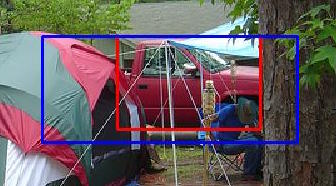
\includegraphics[width=\textwidth]{occluded}
        \end{subfigure}
        \begin{subfigure}[b]{0.4\textwidth}
                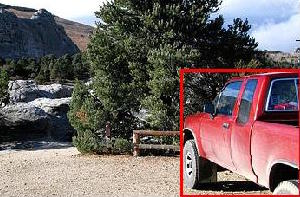
\includegraphics[width=\textwidth]{truncated}
        \end{subfigure}
\caption{Figures illustrating problems with the bounding box annotations on Pascal VOC. The red bounding boxes are the annotations and the blue bounding box illustrates the discrepancy to a real car bounding box.}
\label{fig:trunc}
\end{center}
\end{figure}

\subsection{Handling Truncated and Occluded Objects}\label{sec:trunc}

In experiments on the Pascal VOC 2012 dataset which contains several truncated and occluded objects, the importance of handling truncated and occluded objects effectively became apparent (see figure \ref{fig:trunc}). In this project two approaches were tested to improve  detection of truncated objects.

To detect truncated objects, all levels of the feature pyramid are padded with zeros by half the root size. In DPMver3 the computation of the bounding box overlap requirement during latent search (0.7 overlap) is computed using the root filter box. This discards a lot of truncated examples or leads to wrong component labels as the correct root placement is prohibited by the overlap requirement. An easy fix for this is to clip the root box of truncated examples to image boundaries before computing the overlap. 
It showed that detection performance can be improved further by padding the feature pyramid with the mean hog features computed on positive training examples. An even better performing approach is to augment the feature vectors with an additional truncation bias term  (used in \cite{voc-release4}). This feature term is set to 0 if the feature vector is placed within image boundaries and to 1 if it is outside the image boundaries. This way, the model actually learns which filter regions often are truncated. 

Another observation made on occluded examples was that the minimum bounding box overlap requirement  of 0.7 during latent positive search would often prohibit the correct viewpoint from being chosen. For occluded examples (indicated through annotation) the minimum bounding box requirement was therefore reduced to 0.5.  
As un-occluded and non-truncated object instances should be expected to have "good" bounding boxes in the sense that the model's detection should lead to high bounding box overlap, the penalty term from equation \ref{eq:penalty} has been extended with an overlap penalty term leading to:
\begin{equation}
l(y,z)=(0.5\cdot\mathbbm{1}{ [y_c\neq c] }+0.5\cdot \frac{A_z\cap A_y}{A_z\cup A_y})*\gamma
\end{equation}
Where $A_z$ is the area covered by the hypothesised root filter placement and $A_y$ is the area covered by the annotated bounding box. The intuition behind this was that this enforcing of good bounding box localisation has a similar positive effect as the structured output formulation of \cite{6248075}, while being more flexible as the bounding box overlap is only penalised if the object is in full sight. 